%GNUPLOT: LaTeX picture with Postscript
\begin{picture}(0,0)%
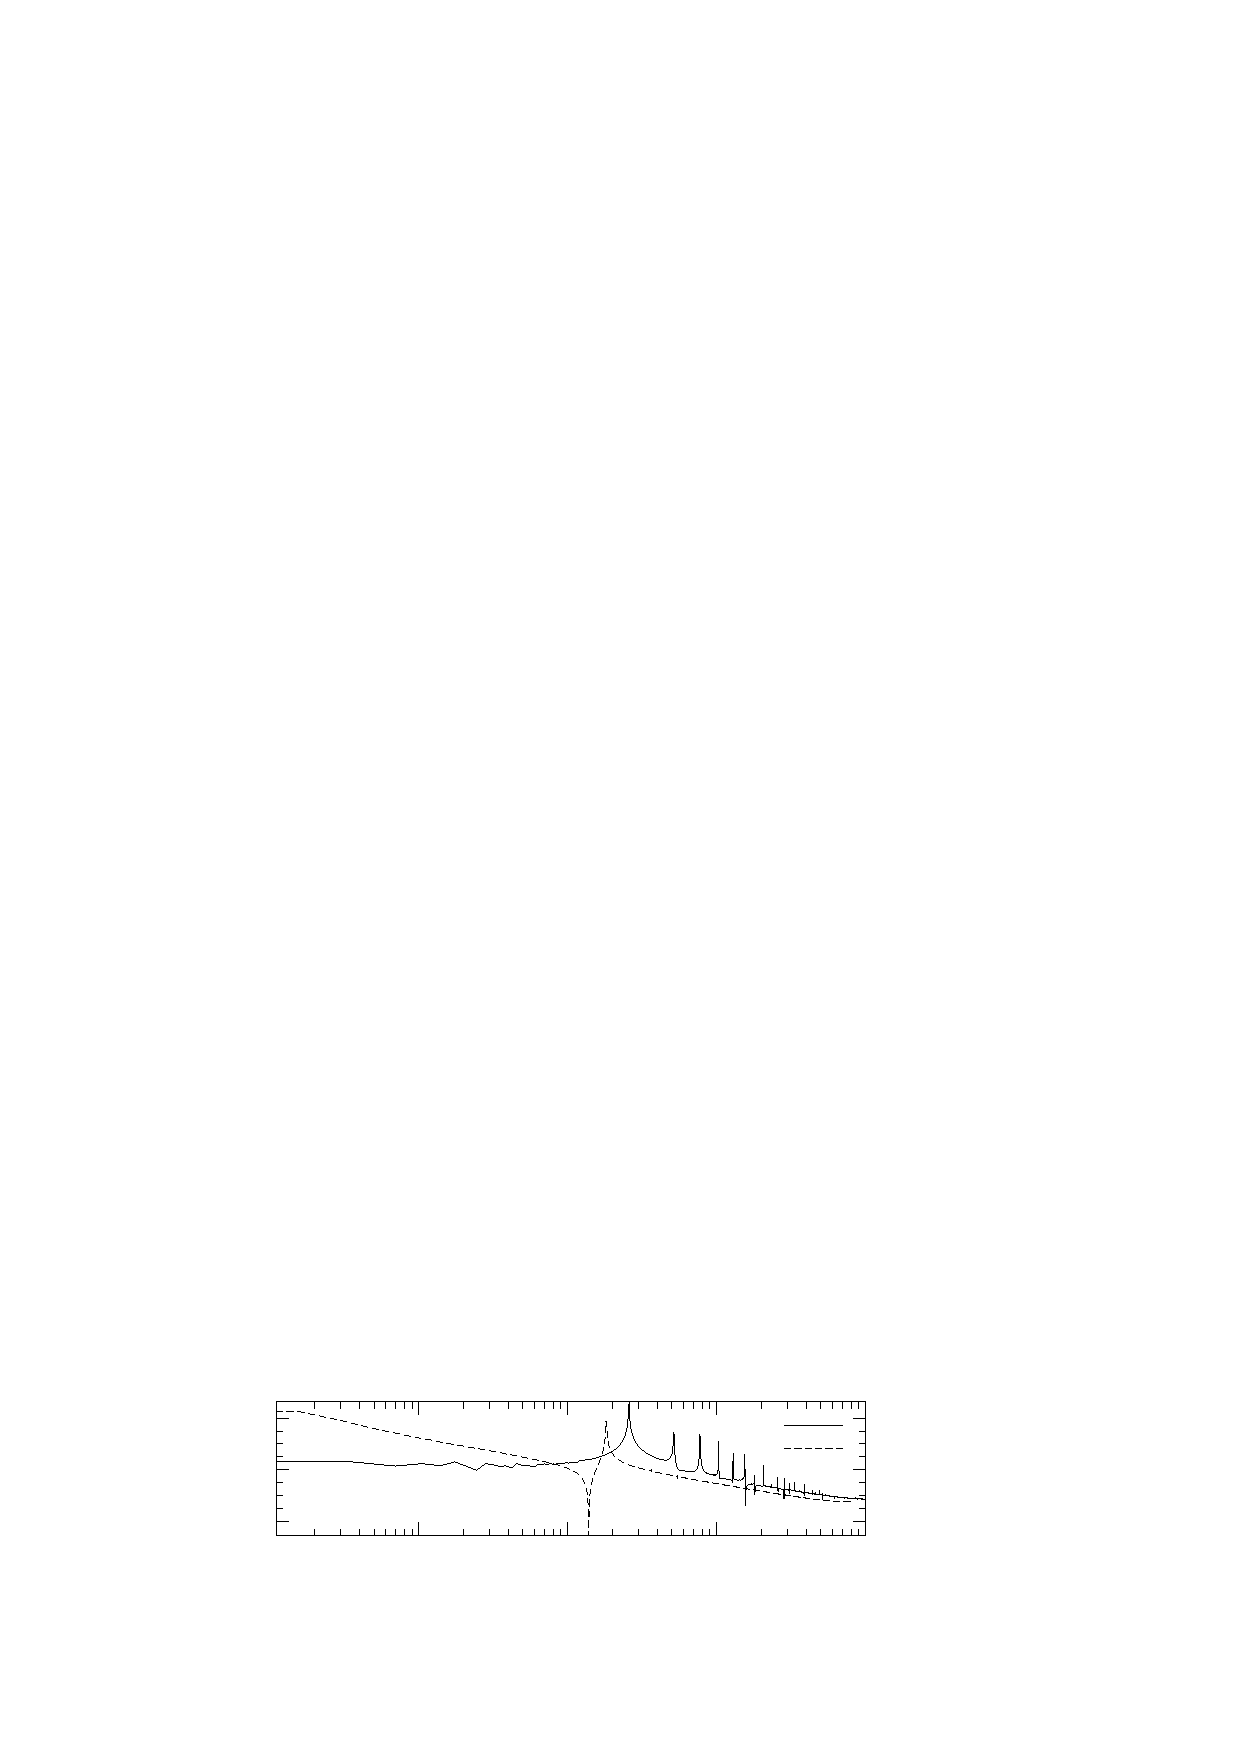
\includegraphics{detalle-frecuencias-rounded-flat-gravity}%
\end{picture}%
\begingroup
\setlength{\unitlength}{0.0200bp}%
\begin{picture}(18000,5400)(0,0)%
\put(2750,1989){\makebox(0,0)[r]{\strut{} 1e-12}}%
\put(2750,3223){\makebox(0,0)[r]{\strut{} 1e-08}}%
\put(2750,4458){\makebox(0,0)[r]{\strut{} 1e-04}}%
\put(6452,1100){\makebox(0,0){\strut{} 0.001}}%
\put(10026,1100){\makebox(0,0){\strut{} 0.01}}%
\put(13601,1100){\makebox(0,0){\strut{} 0.1}}%
\put(17175,1100){\makebox(0,0){\strut{} 1}}%
\put(550,3250){\rotatebox{90}{\makebox(0,0){\strut{}PSD}}}%
\put(10100,275){\makebox(0,0){\strut{}$\omega$}}%
\put(14950,4275){\makebox(0,0)[r]{\strut{}redondeada}}%
\put(14950,3725){\makebox(0,0)[r]{\strut{}plana}}%
\put(600,1000){\rotatebox{0}{\makebox(0,0){\strut{}(b)}}}%
\end{picture}%
\endgroup
\endinput
